\documentclass[tikz,border=5mm]{standalone}

\begin{document}

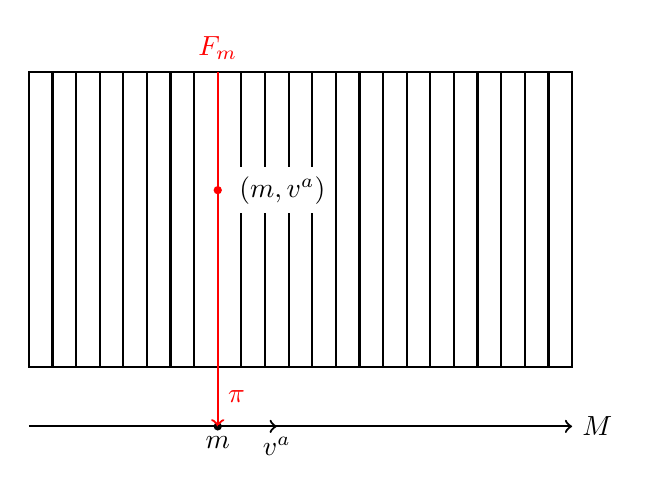
\begin{tikzpicture}[scale=1.5]

% Outer rectangle for the fiber bundle
\draw[thick] (-2.3,0) rectangle (2.3,2.5);

% Base manifold (M)
\draw[thick,->] (-2.3,-0.5) -- (2.3,-0.5) node[right] {$M$};

% Vertical fibers (TM) - denser
\foreach \x in {-2.1,-1.9,...,-0.7} {
    \draw[thick] (\x,0) -- (\x,2.5);
}
\foreach \x in {-0.5,-0.3,...,2.3} {
    \draw[thick] (\x,0) -- (\x,2.5);
}

% Highlight one tangent space TxM
\draw[thick,red] (-0.7,0) -- (-0.7,2.5);
\node[red] at (-0.7,2.7) {$F_m$};
\fill[red] (-0.7,1.5) circle (1pt);
% Labels
\fill (-0.7,-0.5) circle (1pt);
\node[below] at (-0.7,-0.5) {$m$};
\node[fill = white,right] at (-0.6, 1.5){$(m,v^a)$};
% Projection arrow (pi)
\draw[red,->,thick] (-0.7,0) -- (-0.7,-0.5) node[midway,right] {$\pi$};
\draw[->,thick](-0.7,-0.5) -- (-0.2, -0.5) node[below]{$v^a$};

\end{tikzpicture}

\end{document}


